\documentclass[aspectratio=169]{beamer}

\mode<presentation>
{
\usetheme{Madrid}
}

\usepackage{graphics, graphicx}
\usepackage{booktabs}
\usepackage{url}
\DeclareGraphicsExtensions{.pdf,.png,.jpg,.gif}

\title{Linux Beginner Guide}
\author{Jaewoong Lee}
\institute[UNIST]
{
	Ulsan National Institute of Science and Technology
\medskip
\newline
\textit{jwlee230@unist.ac.kr}
}
\date{\today}

\begin{document}
	\begin{frame}
		\titlepage
	\end{frame}

	\begin{frame}
		\frametitle{Contents}
		\tableofcontents
	\end{frame}

	\section{Introduction}
	\begin{frame}
		\frametitle{Introduction}
		
		In this guide, we will discuss about followings:
		\begin{enumerate}
			\item Git
			\item GitHub
			\item GitHub Desktop (\url{https://desktop.github.com})
		\end{enumerate}
	
		As the other program does, Git is basically controlled CLI. But, I don't want to go harder. \\
		In this guide, I will use GUI mainly. 
	\end{frame}

	\begin{frame}
		\frametitle{Git?}
		
		\begin{figure}
			\centering
			
\includegraphics[width=0.4 \linewidth]{figures/git.png}
			\caption{Git}
		\end{figure}
	
		\textbf{Git} is Version Control System (VCS) made by Linus Torvalds. 
	\end{frame}

	\begin{frame}
		\frametitle{VCS?}
		
		\begin{figure}
			\centering
			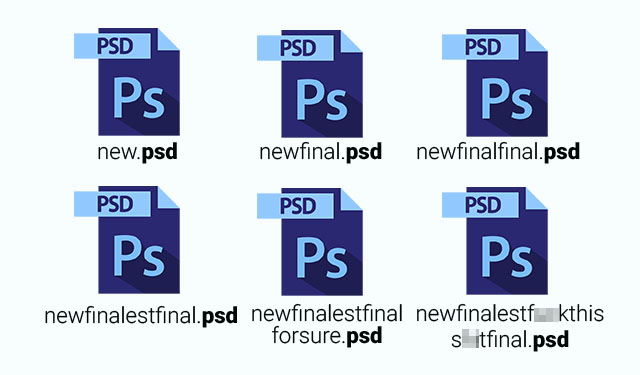
\includegraphics[width=0.4 \linewidth]{figures/final.jpg}
			\caption{Without VCS}
		\end{figure}
	\end{frame}

	\begin{frame}
		\frametitle{VCS? \textit{(Cont.)}}
		
		With VCS, you can get advantages like:
		\begin{itemize}
			\item Revision Control
			\item Version Control
			\item Backup \& Restore
			\item Collaboration
		\end{itemize}
	\end{frame}

	\begin{frame}
		\frametitle{GitHub?}
	\end{frame}

	\section{Basic Step}
	\begin{frame}
		\frametitle{Git Repository}
		
		\textit{Git Repository} means where git save files. There are two types of repository:
		\begin{enumerate}
			\item Remote Repository
			\item Local Repository
		\end{enumerate}
	
		Usually, 
		\begin{enumerate}
			\item you \textit{clone} (download) files from remote repository;
			\item edit files on local repository;
			\item and, \textit{push} (upload) to remote repository.
		\end{enumerate}
	\end{frame}

	\begin{frame}
		\frametitle{Practice 01}
		
		\begin{figure}
			\centering
			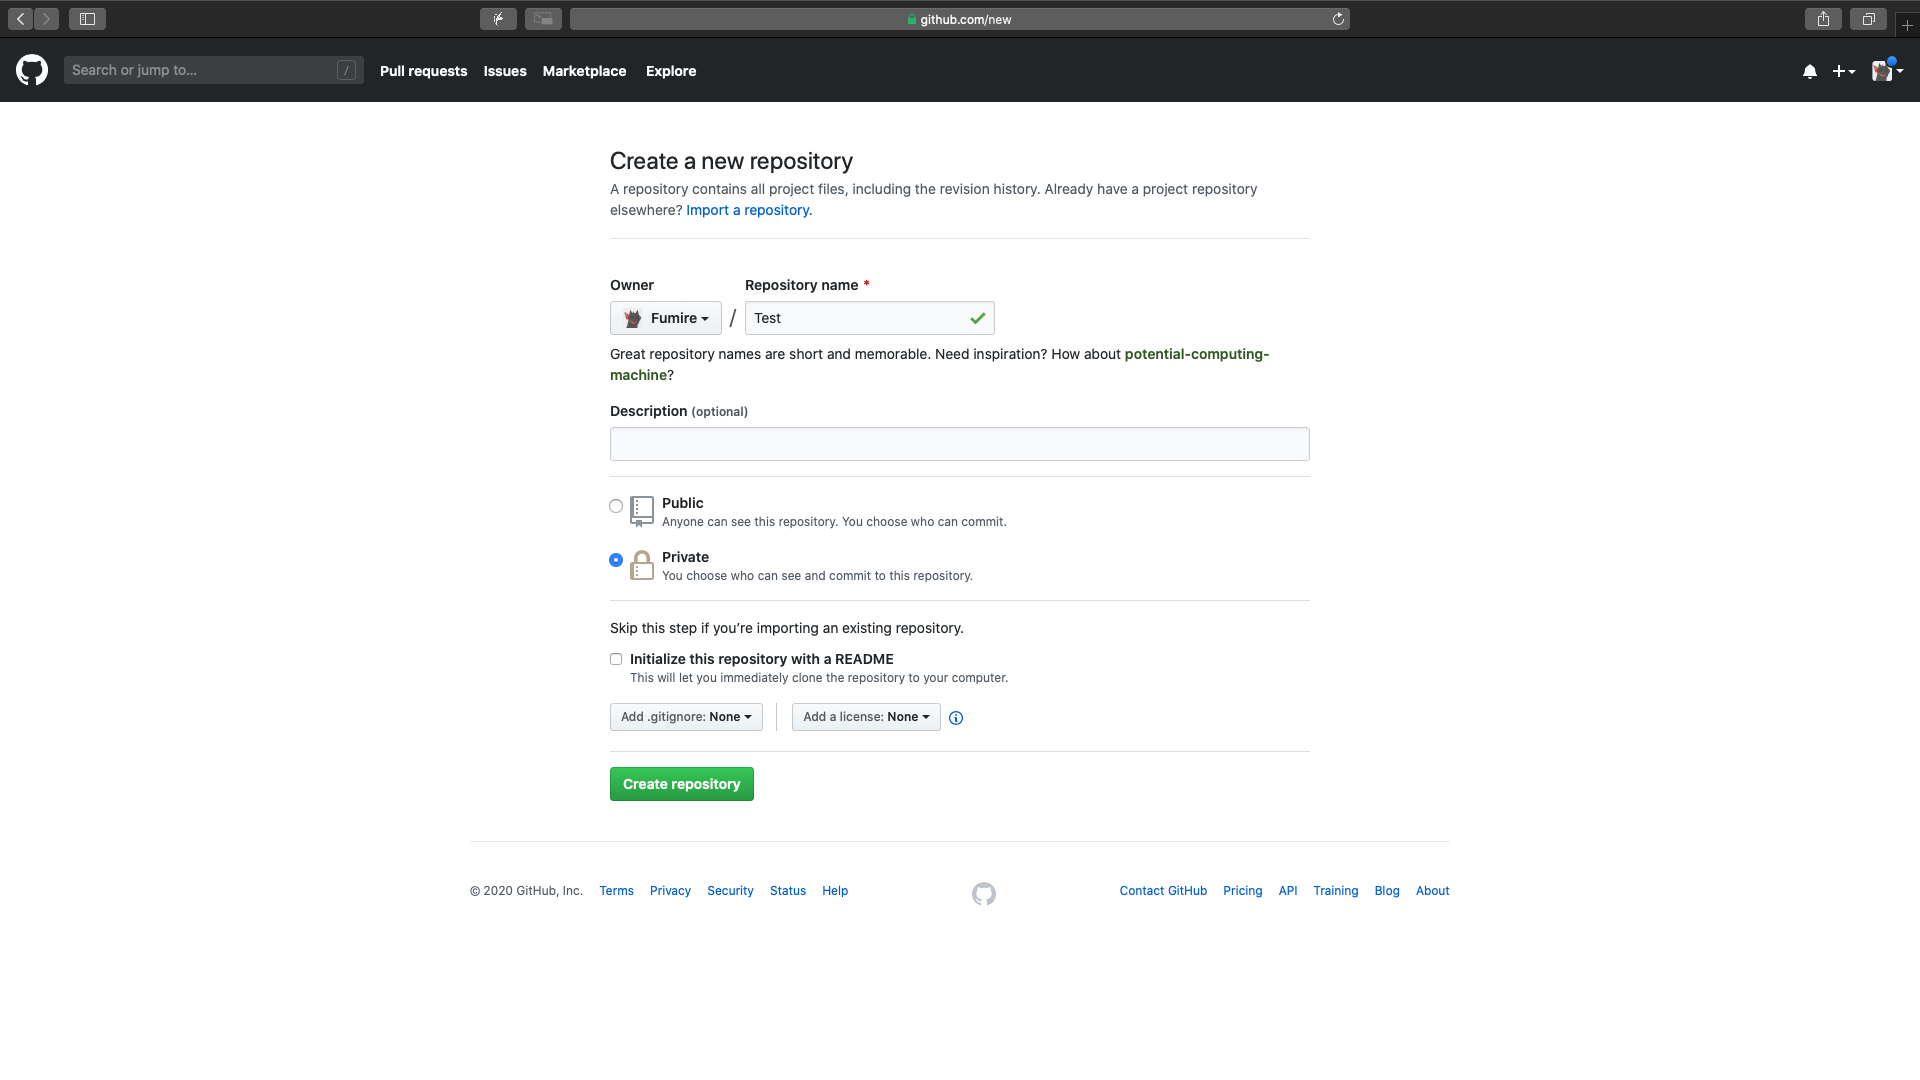
\includegraphics[width=0.6 \linewidth]{figures/1.png}
		\end{figure}
	
		Register \textbf{GitHub}, and make a repository with named 'Test'.
	\end{frame}

	\begin{frame}
		\frametitle{Practice 02}
		
		\begin{figure}
			\centering
			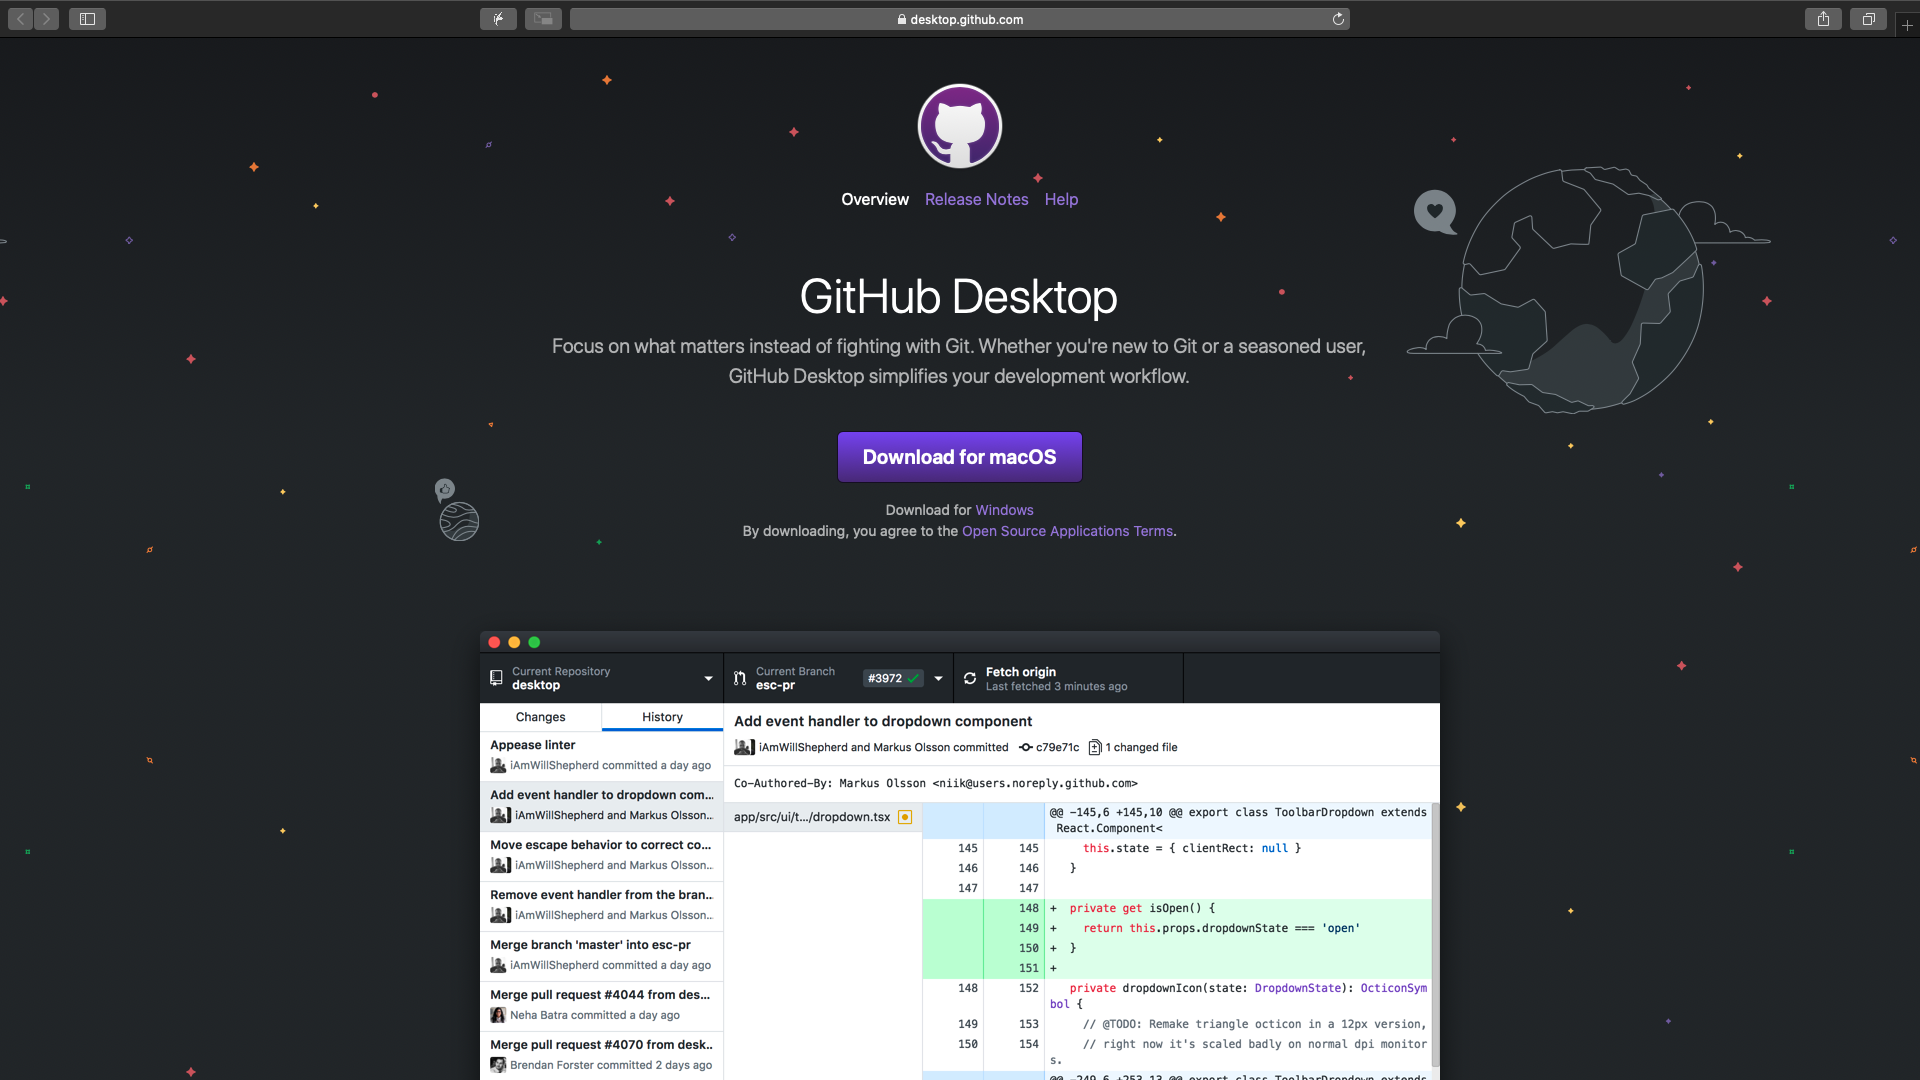
\includegraphics[width=0.6 \linewidth]{figures/2.png}
		\end{figure}
	
		Download \& Install 'GitHub Desktop' which gives GUI control with git. 
	\end{frame}

	\begin{frame}
		\frametitle{Practice 03}
		
		\begin{figure}
			\centering
			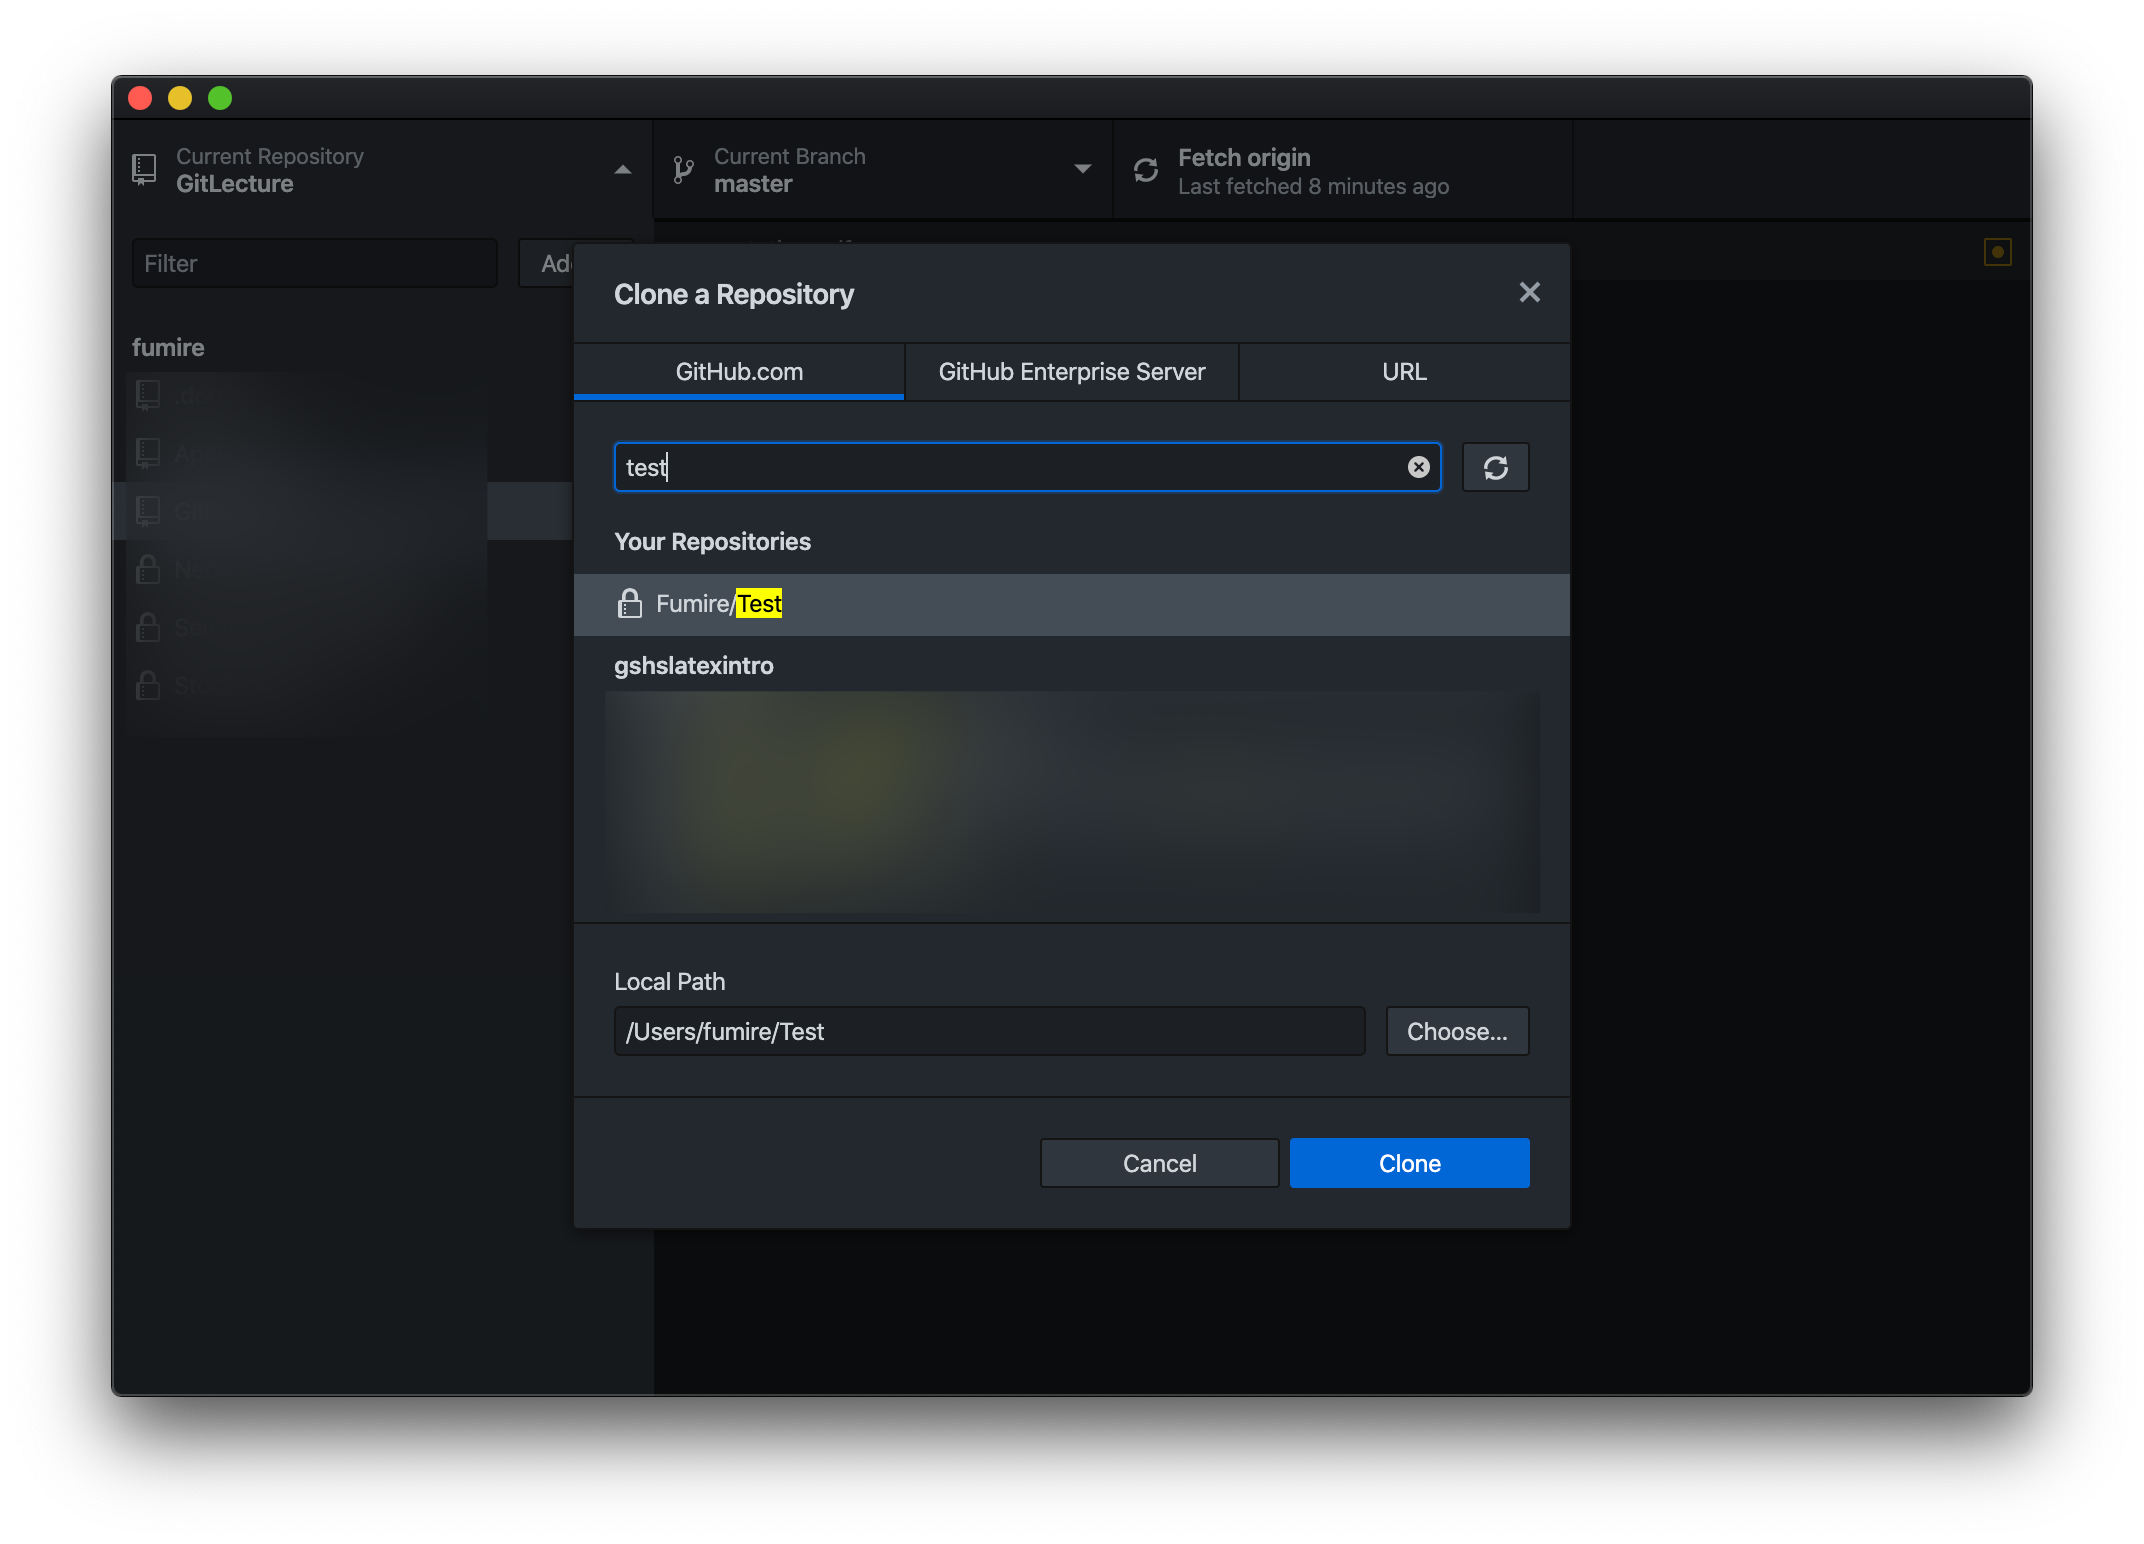
\includegraphics[width=0.5 \linewidth]{figures/3.png}
		\end{figure}
	
		Clone the repository from GitHub as figure. 
	\end{frame}

	\begin{frame}
		\frametitle{Trees}
		
		\begin{figure}
			\centering
			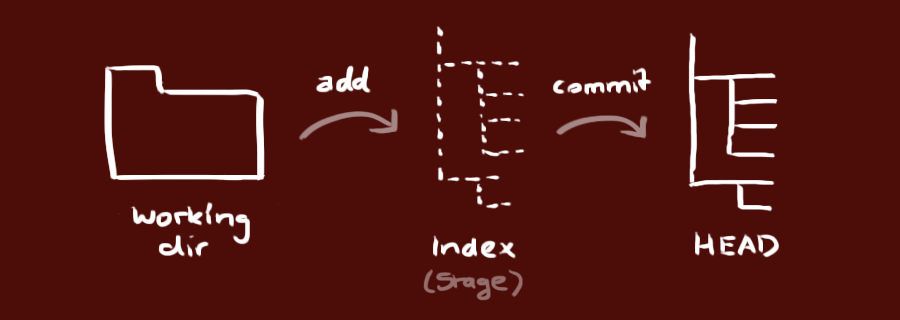
\includegraphics[width=0.5 \linewidth]{figures/trees.png}
		\end{figure}
	
		There are three tree which managed by git. 
		\begin{enumerate}
			\item Working Directory: which consist of real files
			\item Index: staging area (ready area)
			\item HEAD: the final files
		\end{enumerate}
		You can \textit{add} any files from working directory to index. \\
		Also, you could \textit{commit} changes from index to HEAD. \\
		You could add \textit{tag} to commit. 
	\end{frame}

	\begin{frame}
		\frametitle{Practice 04}
		\begin{figure}
			\centering
			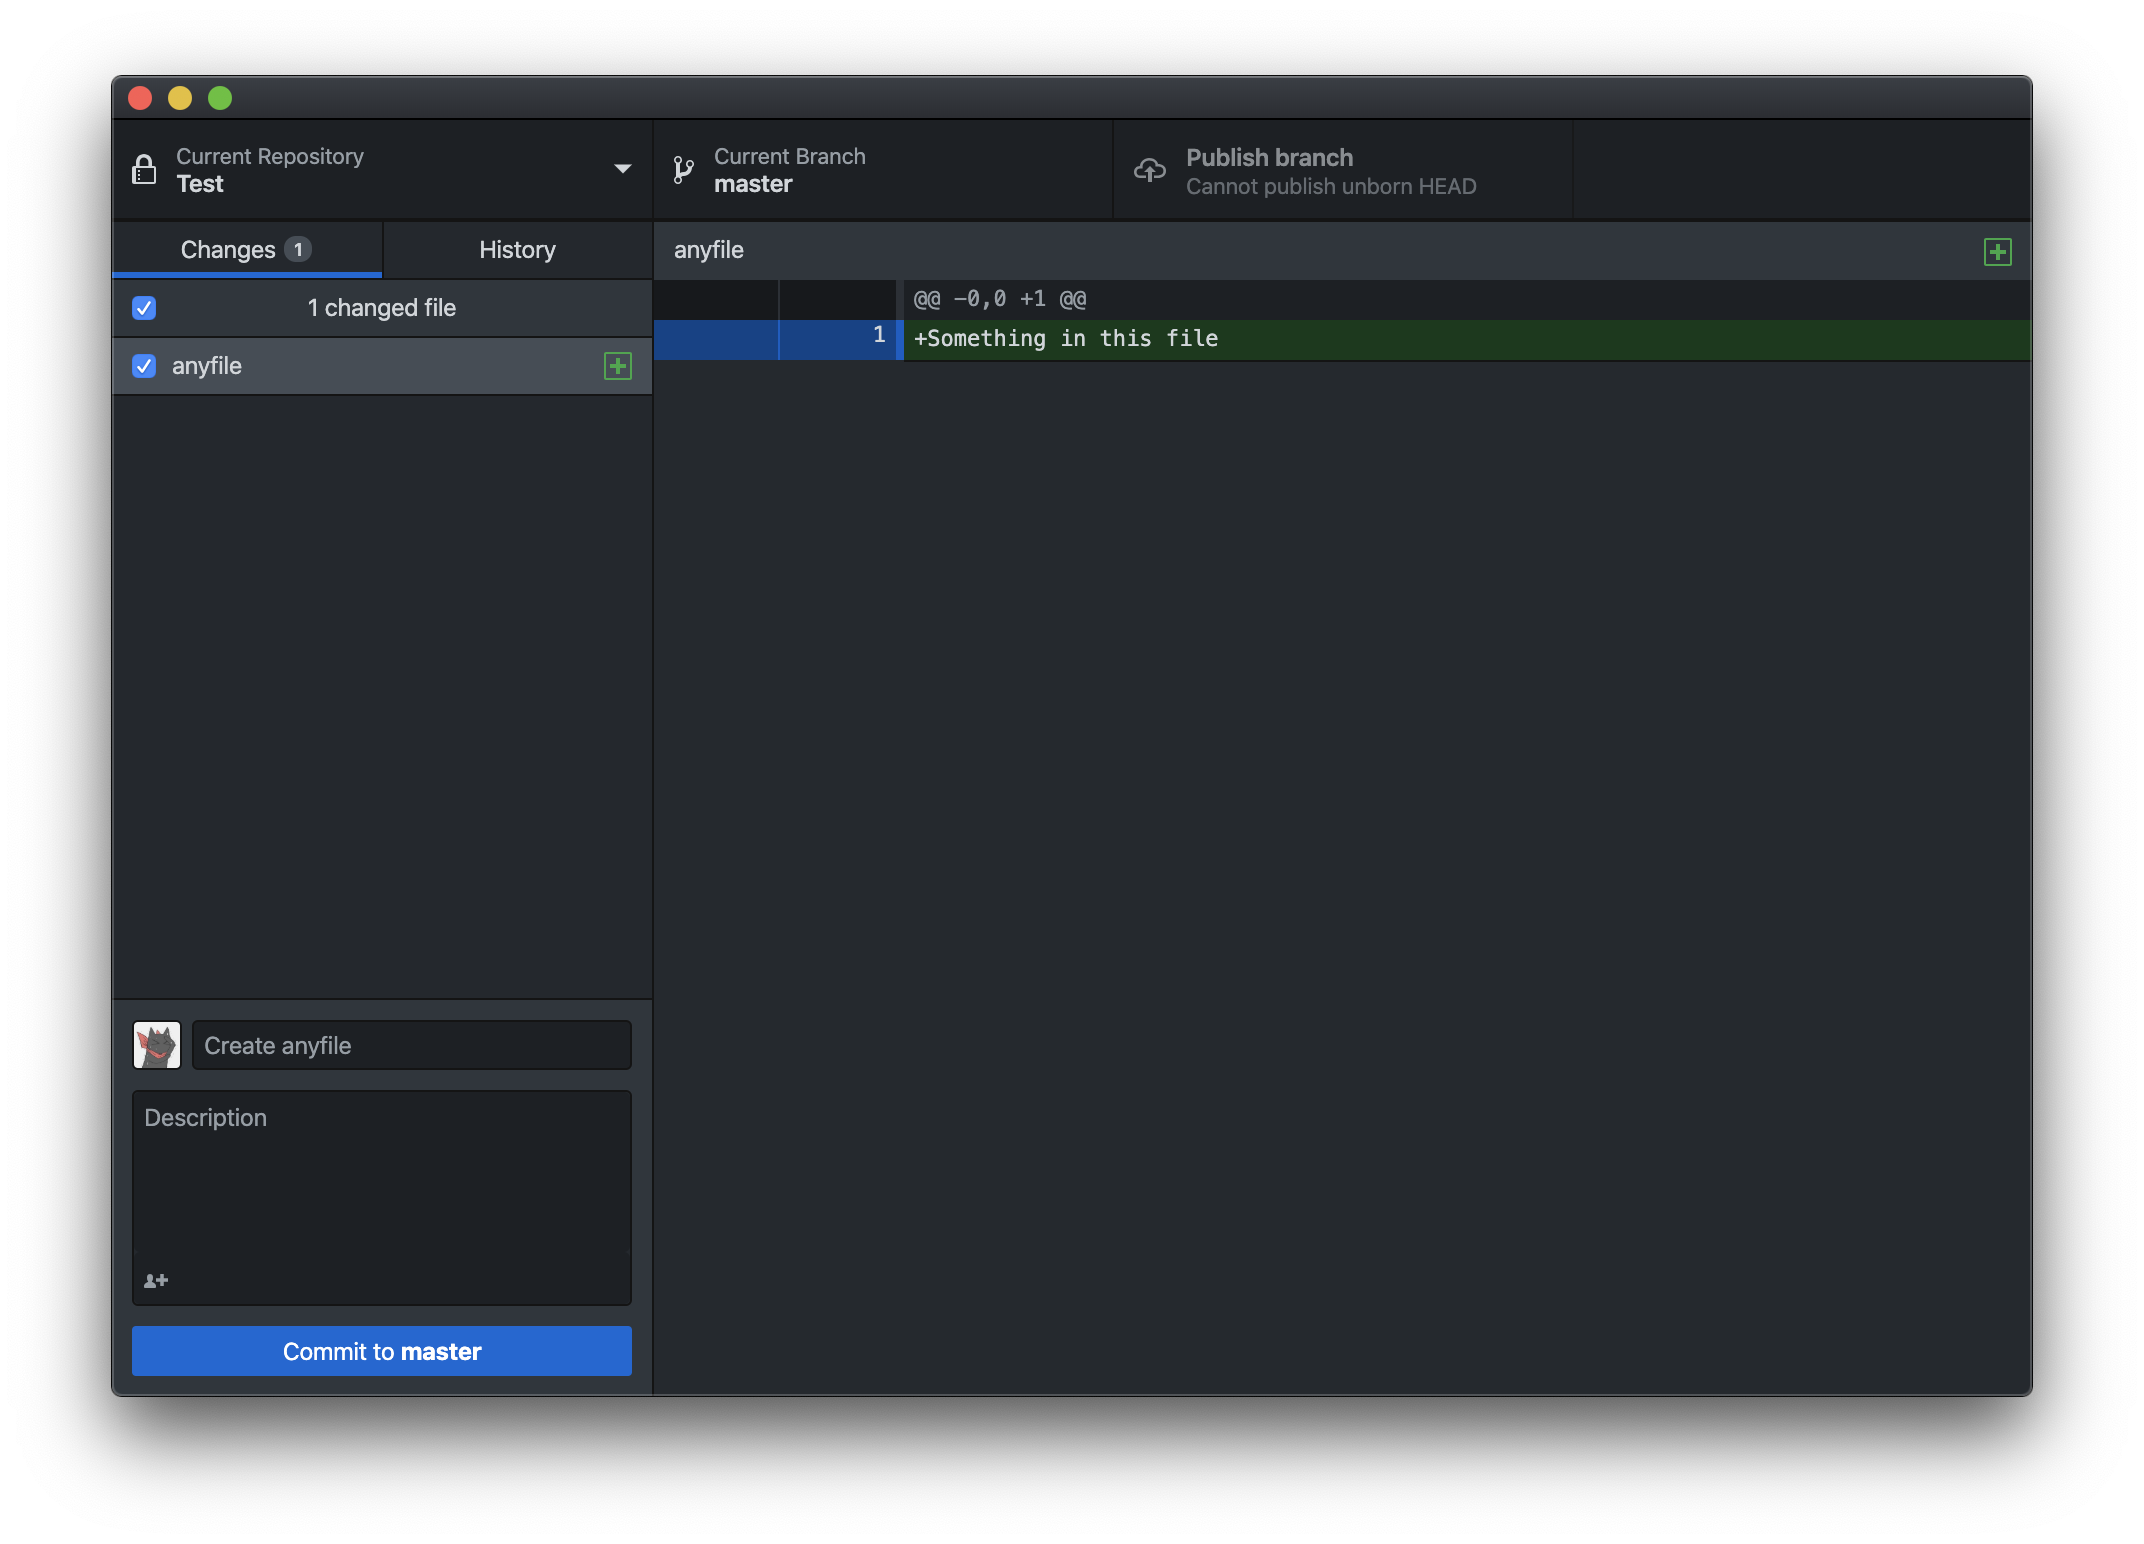
\includegraphics[width=0.5 \linewidth]{figures/4.png}
		\end{figure}
		Add any file to working directory, then GitHub Desktop automatically finds the changes as figures. Commit the changes. 
	\end{frame}

	\begin{frame}
		\frametitle{Push}
		
		However, even you commit the changes, the changes are not applied to remote repository. \\
		The changes are only in local repository. \\
		To apply changes, you should \textit{push} the changes to remote repository. 
	\end{frame}

	\begin{frame}
		\frametitle{Practice 05}
		\begin{figure}
			\centering
			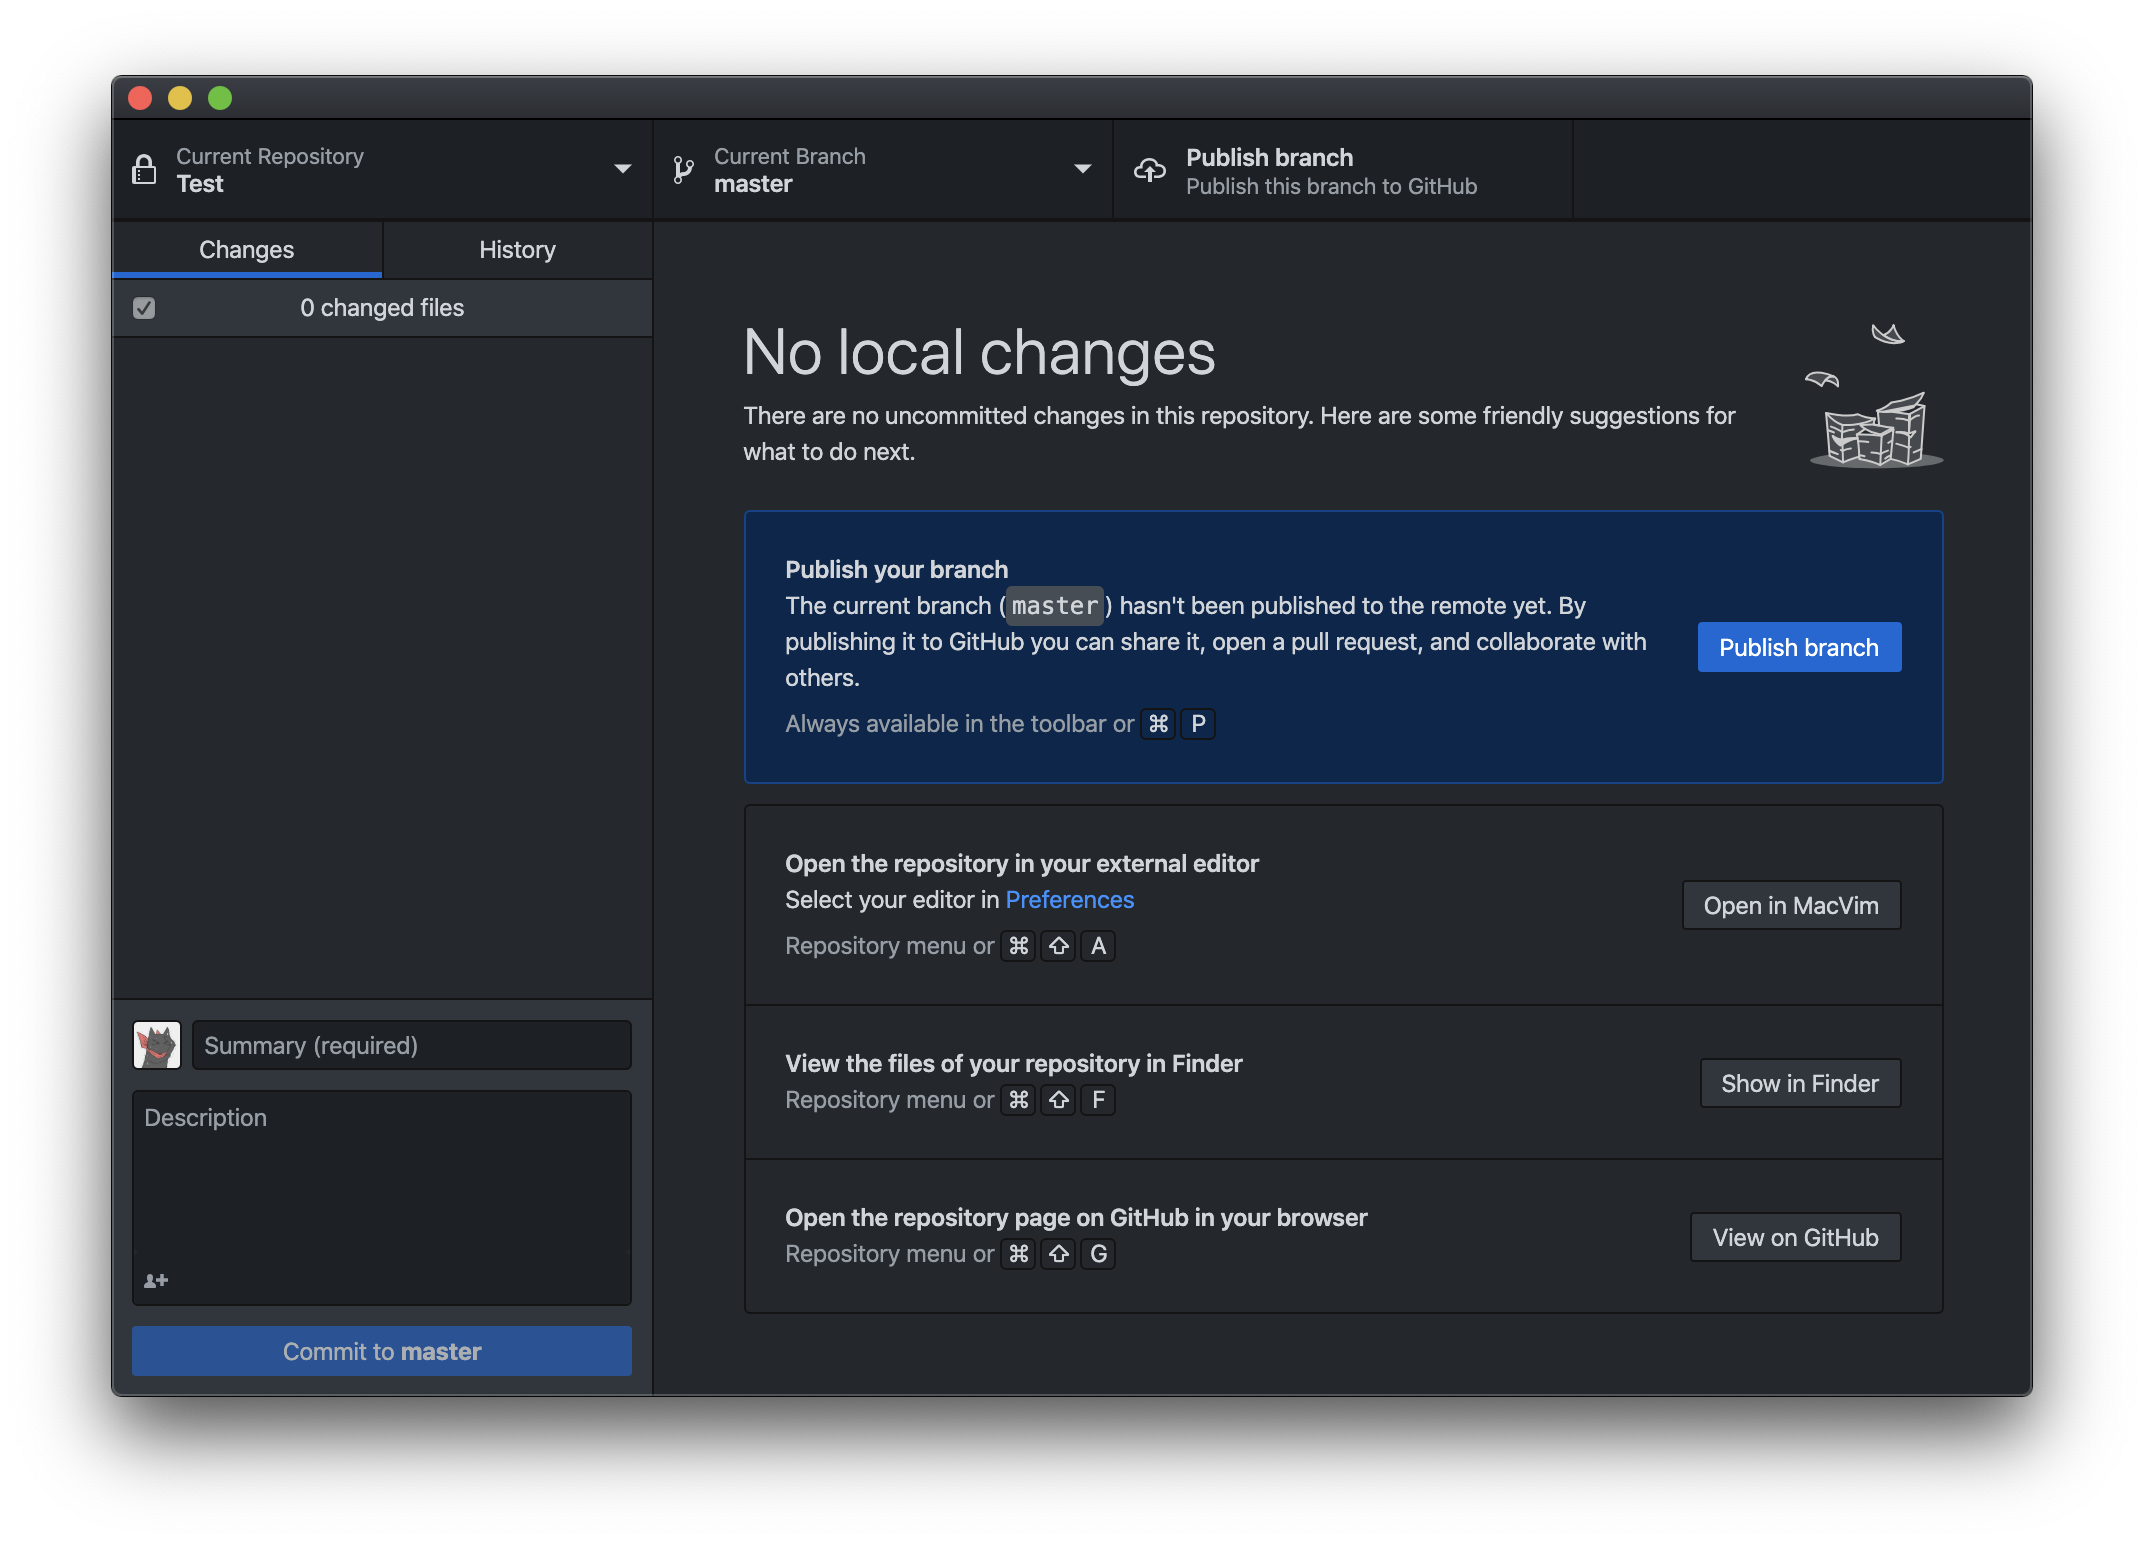
\includegraphics[width=0.5 \linewidth]{figures/5.png}
		\end{figure}
		Let's push the changes to remote repository. 
	\end{frame}

	\begin{frame}
		\frametitle{Branch / Merge}
		You can \textit{branch \& merge} the changes. \\
		The \textbf{master} branch will be automatically generated when creating repository. 
		\begin{figure}
			\centering
			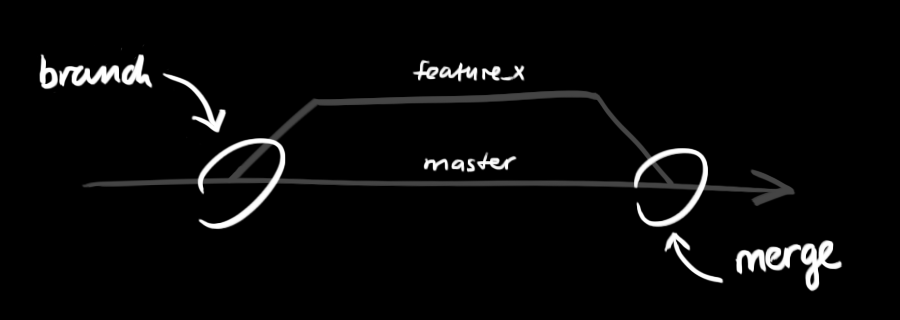
\includegraphics[width=0.5 \linewidth]{figures/branches.png}
		\end{figure}
		You can add/delete branches; and move among the branches. 
	\end{frame}

	\begin{frame}
		\frametitle{Conflict}
		Git automatically try to merge changes. \\
		However, sometimes the \textit{conflict} occurs; in other words, you should solve the twisted. \\
		After you solve the twisted, add/commit the solved as other changes. 
	\end{frame}

	\begin{frame}
		\frametitle{Pull}
		For update as remote directory, you should \textit{pull} the repository. \\
		With \textit{pull} command, the changes of remote directory are \textit{fetched} and \textit{merged}. \\
		Sometimes, as \textit{merging}, conflict can be occurred, and you should solve this. 
	\end{frame}

	\section{Advanced Step}
	\begin{frame}
		\frametitle{Advanced Step}
		After this page, you will get advanced step for git. 
	\end{frame}

	\begin{frame}
		\frametitle{.gitignore}
	\end{frame}

	\begin{frame}
		\frametitle{.gitkeep}
	\end{frame}

	\begin{frame}
		\frametitle{Pull Request}
	\end{frame}

	\begin{frame}
		\frametitle{Fork}
	\end{frame}

	\begin{frame}
		\frametitle{Blame}
	\end{frame}

	\begin{frame}
		\frametitle{References}
		
		\begin{itemize}
			\item Git - The Simple Guide: \url{https://github.com/rogerdudler/git-guide}
		\end{itemize}
	\end{frame}
\end{document}